42. \begin{figure}[ht!]
\center{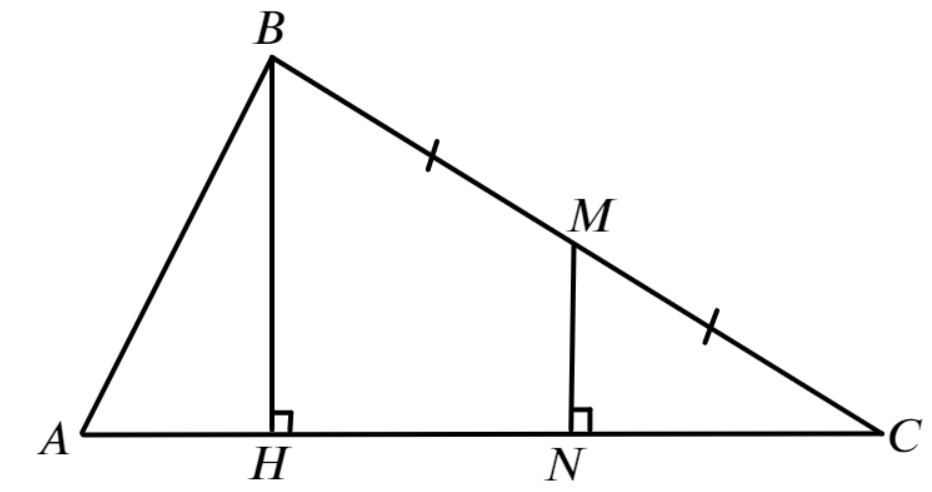
\includegraphics[scale=0.35]{g8-41.png}}
\end{figure}\\
По теореме Пифагора $MN=\sqrt{MC^2-NC^2}=\sqrt{169-25}=12$см. Проведём высоту $BH.$ Треугольники $BHC$ и $MNC$ подобны по двум углам (прямой и общий угол $C$), поэтому $\cfrac{BH}{MN}=\cfrac{BC}{MC}=2\Rightarrow BH=2\cdot12=24$см. Тогда $S_{\Delta ABC}=\cfrac{1}{2}BH\cdot AC=\cfrac{1}{2}\cdot24\cdot(19+5)=288\text{ см}^2.$\\
